\documentclass[prl,aps,twocolumn,floatfix,amsmath,amssymb,superscriptaddress,tightenlines]{revtex4}
\usepackage{graphicx}% Include figure files
\usepackage{epstopdf}
%\usepackage{amsmath}
\usepackage{amsfonts}
\usepackage{bm}
%\bibliographystyle{prsty}
\begin{document}

\date{\today}
\title{Valence Bond and von Neumann Entanglement Entropy in Heisenberg Ladders}
\author{Ann B. Kallin}
\affiliation{Department of Physics and Astronomy, University of Waterloo, Ontario, N2L 3G1, Canada} 

\author{Iv\'an Gonz\'alez}
%\affiliation{Fundaci\'on Centro Tecnol\'ogico de Supercomputaci\'on de Galicia (CESGA), Santiago de Compostela, Spain}
\affiliation{Centro de Supercomputaci\'on de Galicia, %(CESGA), 
Avda.~de~Vigo~s/n, E-15705 Santiago de Compostela, Spain}

\author{Matthew B. Hastings}
\affiliation{Microsoft Research, Station Q, CNSI Building, University of California, Santa Barbara, CA, 93106.}

\author{Roger G. Melko}
\affiliation{Department of Physics and Astronomy, University of Waterloo, Ontario, N2L 3G1, Canada} 

\begin{abstract}

\end{abstract}
\maketitle

%\newpage

{\it Introduction.}-- Entanglement has arisen in condensed matter physics
as a new paradigm for the study of correlations in a system.  Measurements
of entanglement between separate subregions, chiefly using entropic
quantities, have an advantage over traditional two-point correlation
functions in that they encode the total amount of information shared
between two subregions without the possibility of missing ``hidden''
correlations \cite{wolf}.  Such hidden correlations may occur in some
quantum groundstates,  in particular the important example of spin liquid
states, where two-point correlation functions decay at large lengthscales.
However, it is well known that a type of topological order may exist in
spin liquids, which may be quantified in a ``topological entanglement
entropy'', a property of the groundstate wavefunction \cite{ KP, LW}.
This and other entropic measures are typically discussed in the context of
the von Neumann entanglement entropy, which for a system partitioned into
two regions A and B, quantifies the amount of entanglement of A with B as
--This line, and those below, will be ignored-- \begin{equation} S^{\rm
VN}_A = - {\rm Tr} [ \rho_A \ln \rho_A ]. \label{vNEE} \end{equation}
Here, the reduced density matrix $\rho_A = {\rm Tr}_B | \psi \rangle
\langle \psi |$ is obtained by tracing out the degrees of freedom
associated with the region B.

The von Neumann (VN) entanglement entropy (EE) has a well-defined and
oft-studied set of analytical properties in interacting quantum systems.
In one dimension (1D), exact analytical results are known from conformal
field theories (CFT); they show that, away from special critical points,
the VN EE between A and B scales according to the size of the boundary.
This so-called {\it area law} is also believed to hold in many
groundstates of two dimensional (2D) interacting quantum Hamiltonians,
although few exact results are available \cite{ALreview}.  Of particular
importance, the existence of an area law has consequences in the
rapidly-advancing field of computational quantum-many body theory: it is
known that if the groundstate of a one-dimensional Hamiltonian satisfies
an area law, then this state is well approximated by a Matrix Product
State (MPS).  Tensor-network extension of such MPS states are the basis
for a new promising class of numerical algorithms that may push our
abilities to simulate two-dimensional (2D) quantum systems past that
allowed by quantum Monte Carlo (QMC) technologies, which are hampered by
the notorious fermionic sign problem.  However, it is believed that 2D
states which lend themselves to accurate approximation by such methods
must also obey an area law.

%\begin{figure} { 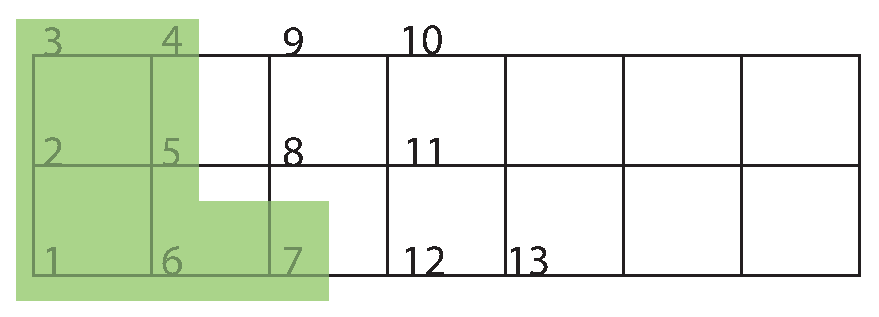
\includegraphics[width=2.4in]{ladder.eps}
%\caption{(color online) A three-leg ladder.  The site labels $x$ indicate
%the order in which DMRG sweeping takes place, which is also the index
%order by which entanglement entropy is measured.  The blue box labels
%sites in the region A, with $x=7$.  \label{ladder}}} \end{figure}

Thus the question of an area law in the groundstates of 2D quantum systems
is of the utmost importance for the development of new simulation
techniques.  Paradoxically, it is also a quantity that is difficult to
measure in 2D systems, due to the fact that QMC techniques (currently the
only scalable method capable of unbiased 2D simulations) do not have
direct access to the groundstate wavefunction $| \psi \rangle$, required
to construct the VN EE.  In response to this, several authors \cite{Alet,
Chh} has recently introduced the concept of {\it valence bond} (VB)
entanglement entropy, defined for an SU(2) symmetric spin system as
\begin{equation} S^{\rm VB}_A = \ln(2) \cdot \mathcal{N}_A, \label{VBEE}
\end{equation} where $ \mathcal{N}_A$ is the number of EPR spin singlets
${( |\uparrow \downarrow \rangle - | \downarrow \uparrow
\rangle)/\sqrt{2}}$ crossing the boundary between regions A and B.  Unlike
the VN EE, the VB EE can be accessed very easily in the valence-bond basis
projector QMC method recently proposed by Sandvik \cite{Sandvik}.  As
demonstrated in Refs.~\cite{Alet,Chh}, the VB EE has many properties in
common with the VN EE, in particular the relationship $S_A = S_B$, and the
fact that $S^{VB}_A=0$ for regions ``un-entangled'' by valence bonds.
Further, a comparison of the scaling of the VB EE for a (critical) 1D spin
1/2 Heisenberg chain shows good agreement with analytical results known
from conformal field theory (CFT), which we discuss more below.  What is
particularly striking about the results presented in Refs.~\cite{Alet,Chh}
is the extension of their work to the 2D isotropic Heisenberg model, which
displays a {\it multiplicative} logarithmic correction to the area law.
This multiplicative log correction was attributed to algebraically
decaying correlations \cite{Chh} and gapless modes \cite{Alet}.  If this
property were to be shared by the VN EE, it could have the consequence
that the 2D Neel groundstate can not be approximated by a tensor-network,
and is therefore not amenable to simulation techniques based on the MPS
framework
 
In this paper, we compare the VB EE calculated by valence-bond QMC to the
VN EE accessible through large-scale density-matrix renormalization group
(DMRG) measurements on the Heisenberg model on multi-leg ladder
geometries.    We show that in 1D, contrary to initial results presented
in Refs.~\cite{Alet,Chh}, the CFT central charge calculated by scaling the
VN EE (confirmed with DMRG to converge to $c=1$) does not converge to the
expected result when calculated by scaling the VB EE.  On multi-leg
ladders, it becomes clear that the VB EE is always greater than the VN EE,
a trend which grows rapidly with the number of legs $N$.  Finally, a
comparison of the area law defined by bisecting the multi-leg ladders
shows a clear logarithmic correction for the VN EE, $S^{VB}_A /N = N \ln
N$ (in agreement with Refs.~\cite{Alet,Chh}), however for data up to
$N=7$, the VN EE as calculated by DMRG convincingly shows a scaling of
$S^{VB}_A /N = N$, the expected area law.

{\it Model and Methods.}-- We consider the spin 1/2 Heisenberg
Hamiltonian, given by \begin{equation} H = J \sum_{\langle i j \rangle}
{\mathbf S}_i \cdot {\mathbf S}_j \label{ham} \end{equation} where the sum
is over nearest-neighbor sites.  Geometries studied are 1D chains, and
multi-leg ladders with length $L$ and number of legs $n$.  
%Many properties of this model on open-boundary ladders with $n$ legs has
%been exhaustively studied.  Of importance, it is known that a spin gap
%exists for even-$n$ ladders in the limit of $L\rightarrow \infty$,
%whereas odd-$n$ ladders behave somewhat more like quasi-1D  systems with
%spin $n/2$ and, from Haldane's conjecture, are therefore gapless.  
We employ two complementary numerical techniques in our study of EE on
ladder geometries, namely the valence-bond basis QMC and DMRG, both of
which give {\it unbiased} approximations to the ground state of the
Hamiltonian at zero temperature, and results from both of which can be
compared directly to one another.  The VN EE is naturally accessible
through the DRMG ``sweeping'' algorithm~\cite{White92, Scholl05}.  At each
step of the algorithm, the wavefunction of the system is approximated by
keeping only the states with largest coefficients in the Schmidt's
decomposition for subregions A and B. To find the basis entering the
Schmidt's decomposition for subregion A, the reduced density matrix
$\rho_A$ is calculated and diagonalized, thus allowing easy calculation
of Eq.~\ref{vNEE}. The truncation of the basis implies that only an upper
bound for $S^{VN}_{A}$ is calculated, so care must be taken to ensure
that enough of the eigenvalue spectrum is included to converge the VN EE
to sufficient accuracy; typically the number of states required is larger
then that needed to converge the energy alone.

The VB EE can be calculated using the valence-bond basis QMC proposed by
Sandvik in 2005 \cite{Sandvik}.  The valence-bond basis QMC algorithm that
we use is the simple single-projector method, with lattice geometries
constructed to match those given by the DMRG algorithm.  The ground state
of the system is projected out by repeated application of a list of bond
operators on nearest neighbor sites of the ladder.  A number of bond
operators ($r$) are changed each step and the change is accepted with a
probability depending on the number of nearest neighbor bonds in the
resulting valence bond states.  Measured quantities such as energy or
valence bond entanglement entropy are then calculated by a weighted
average over all the valence bond states obtained by this procedure.

\begin{figure} {
%
\includegraphics[width=3.2in]{fig1_inset.eps}

\includegraphics[width=3.3in]{4-panelFIG1.eps} \caption{(color online)
Valence bond (VB) and von Neumann (VN) entanglement entropies (EE) for 1D
Heisenberg model with (left panels) periodic boundary conditions (PBC),
and (right panels) open boundary conditions (OBC). Upper panels show the
entropies as a function of the conformal distance $x'$ for 100-site chains
(see text). Lower plots show the values for the central charge $c$,
obtained by fitting the numerical data to the conformal field theory
result, for several chain lengths. For PBC (left panel), $c$ is plotted as
a function of inverse system size. For OBC (right panel), boundary effects
make the fits depend on the number of sites included in the fit, $z$. To
bypass these effects we plot $c$ as a function $z$ for each $L$. Here, $z$
is systematically decreased by removing points from the {\it outside} ends
of the open-boundary chain. $c$ is illustrated for the VN EE (closed
symbols) and the VB EE (open symbols) for system sizes $L=64$ (circles),
$L=100$ (squares), $L=128$ (diamonds), and $L=200$ (triangles)
\label{1D}}} \end{figure}

{\it One-dimensional chain.}-- We consider first the case of 1D Heisenberg
chains. We employ both open (OBC) and periodic (PBC) boundary conditions
with both DMRG and QMC, in order to study the VN and VB entanglement
entropies (PBCs typically have poorer convergence properties than OBCS
within DMRG and more states must be kept in each truncation). 
% I will delete this sentence between brakets if needed: this is well
% known and does not bring much to the paper discussion
DMRG algorithm requires both subregions A and B to be topologically
connected, so in 1D the bipartition is defined by a site $x$ with sites
within the interval $[1,x]$ ($[x+1,L]$) belonging to subregion $A$ ($B$),
$L$ being the lenght of the chain. We stress that the QMC and DMRG results
are on the same geometry and Hamiltonian, and reproduce the same ground
state energies; the remaining figures in the paper can be considered as
exact comparisons between the VB and VN EE. 

Hamiltonian~(\ref{ham}) in 1D is known to be critical and therefore can be
mapped to a 2D classical Hamiltonian at its critical point, which in turn
can be described within conformal field theory (CFT) in the limit
$L\to\infty$.  To address chains of finite lengths one can use the
conformal mappings $x\to x'=L/\pi \sin(\pi x / L)$ for PBC, and $x\to
x'=2L/\pi \sin(\pi x / L)$ for OBC. VN EE calculations within
CFT~\cite{Cardy, Scholl06} obey $S^{VN}(x)= c/3 \ln(x') + S_1$ in the PBC
case, and $S^{VN}(x)= c/6 \ln(x') + \ln(g)+S_1/2$ in the OBC case, where
$c$ is the central charge of the CFT, $S_1$ is a model-dependent constant,
and $g$ is Ludwig and Affleck's universal boundary
term~\cite{AffleckAndLudwig}.

Figure~\ref{1D} illustrates simulation results in both cases, the left
(right) panels corresponding to PBC (OBC). In Refs.~\cite{Alet, Chh}, VB
EE calculated from QMC was compared to the CFT result, and a good fit to
a central charge of $c=1$ was found for both cases.  In Fig.~\ref{1D} we
compare this result to the VN EE calculated from the DMRG.  
In the left panels of Fig.~\ref{1D}, both the VN and VB entropies are seen
to fit well to the CFT result, although the VN EE is greater than the VB
EE. The regression fit shows very good convergence with the CFT central
charge prediction for the VN EE , while the VB EE fit yields a lower than
predicted result. {\it (Should I include this?) It is possible the VB EE
data is not sufficiently converged which would could give results below
the CFT predicted value, however data from Refs.~\cite{Alet,Chh} bears
similar results. }

In the right panels of Fig.~\ref{1D}, both the VN and VB EE are seen to
split into two branches, the upper (lower) corresponding to an odd (even)
number of lattice sites in $A$.  This reflects a well-known
``dimerization'' effect induced by OBC~\cite{Ian1}.  Notice that contrary
to the PBC case, the VN EE is now \textit{smaller} than the VB EE. A
regression fit of the lower branch to the form $c/6 \ln {x'}$ (inset)
shows excellent convergence of the VN EE to the central charge predicted
by CFT, $c=1$, once finite-size effects and the proximity of the data to
the open boundaries is taken into account.  In contrast, the VB EE fit
deviates significantly from the CFT result for larger system sizes, give
$c>1$ when all or most data is included in the fit, and $c<1$ as data is
systematically excluded from the fit (data closest to the open boundary is
removed first).

{\it Multi-leg ladders.}-- Moving away from the one dimensional chain, one
can add ``legs'' to the lattice in a systematic way. 

{\it Area law in multi-leg ladders.}--  Given the ground state of a
quantum many-body system in 2D, the question of whether the entanglement
entropy fulfills and "area" (boundary) law is in general a difficult one
to answer.  However from a simulation perspective this question is of
utmost importance, since tensor-network generalization of MPS techniques,
such as PEPS, produce states that satisfy the area law by construction.
Thus in order to simulate, for example, the N\'eel groundstate of the 2D
Heisenberg model accurately with such methods depends critically on
whether or not the entanglement entropy of the N\'eel state obeys an area
law.  Refs.~\cite{Alet,Chh} examined this issue using the VB EE, and found
clear multiplicative logarithmic corrections to the area law in the N\'eel
state, which was tentatively attributed to gapless Goldstone modes and
algebraically decaying correlations.  

We can address this question using our data for the VB and VN EE alluded
to in the above section on multi-leg ladders.  That is, we chose a lattice
geometry such that subregion A is rectangular, cutting a multi-leg ladder
cleanly across a rung, such that the ``area'' separating region A and B is
equivalent to the number of legs in the ladder $N$.  We chose this area A
to contain contain $2N^2$ sites ...{\bf Matt: do we want to spell out the
argument involving the sum over quasi-1D modes?  I think we will have
room}.

Fig.~\ref{zigzag} illustrates the simulation results for $N$-leg ladders.
Plotting $S_A/N$ versus $N$ on a log scale, one sees that we reproduce the
multiplicative logarithmic correction to the VB area-law, in agreement
with Refs.~\cite{Alet,Chh}.  However, the linear slope is not present in
the plot of the VN EE data from the DMRG, which convincingly approaches a
constant for large $N$.  Clearly, the VN EE suggests that the area law is
indeed obeyed in the N\'eel groundstate, leading one to conclude that the
multiplicative logarithmic correction is an artifact of the VB EE.

%Despite the importance of adherence to the area law in tensor-network
%generalization of MPS techniques, it is still not yet known whether the
%2D isotropic Heisenberg ground state does obey the area law.  The results
%from Refs.~\cite{Alet,Chh} for the VB EE in 2D indicate a multiplicative
%logarithmic corrections to the area law.  We find it necessary to address
%whether the same logarithmic correction exists in the VN EE.
%Fig.~\ref{zigzag} shows the VB EE and VN EE for ladders with N legs.  The
%lattice geometry is chosen such that subregion A contains $2N^2$ sites
%and is always rectangular.  It is clear that Fig.~\ref{zigzag} shows a
%logarithmic correction to the area law for VB EE, in agreement with
%Refs.~\cite{Alet,Chh}.  However, in the case of the VN EE, the data
%approaches a constant value and shows no correction to the area law.

\begin{figure} { 
\includegraphics[width=3in]{FIG2.eps} \caption{(color
online) Valence Bond and von Neumann entanglements entropies for a 4-leg
ladder system with 100 sites per leg.  In this and similar geometries, $x$
is the site index of the ladder, defined using the usual DMRG
sweeping-convention (inset lower left).  \label{ladder}}} \end{figure}

\begin{figure} { 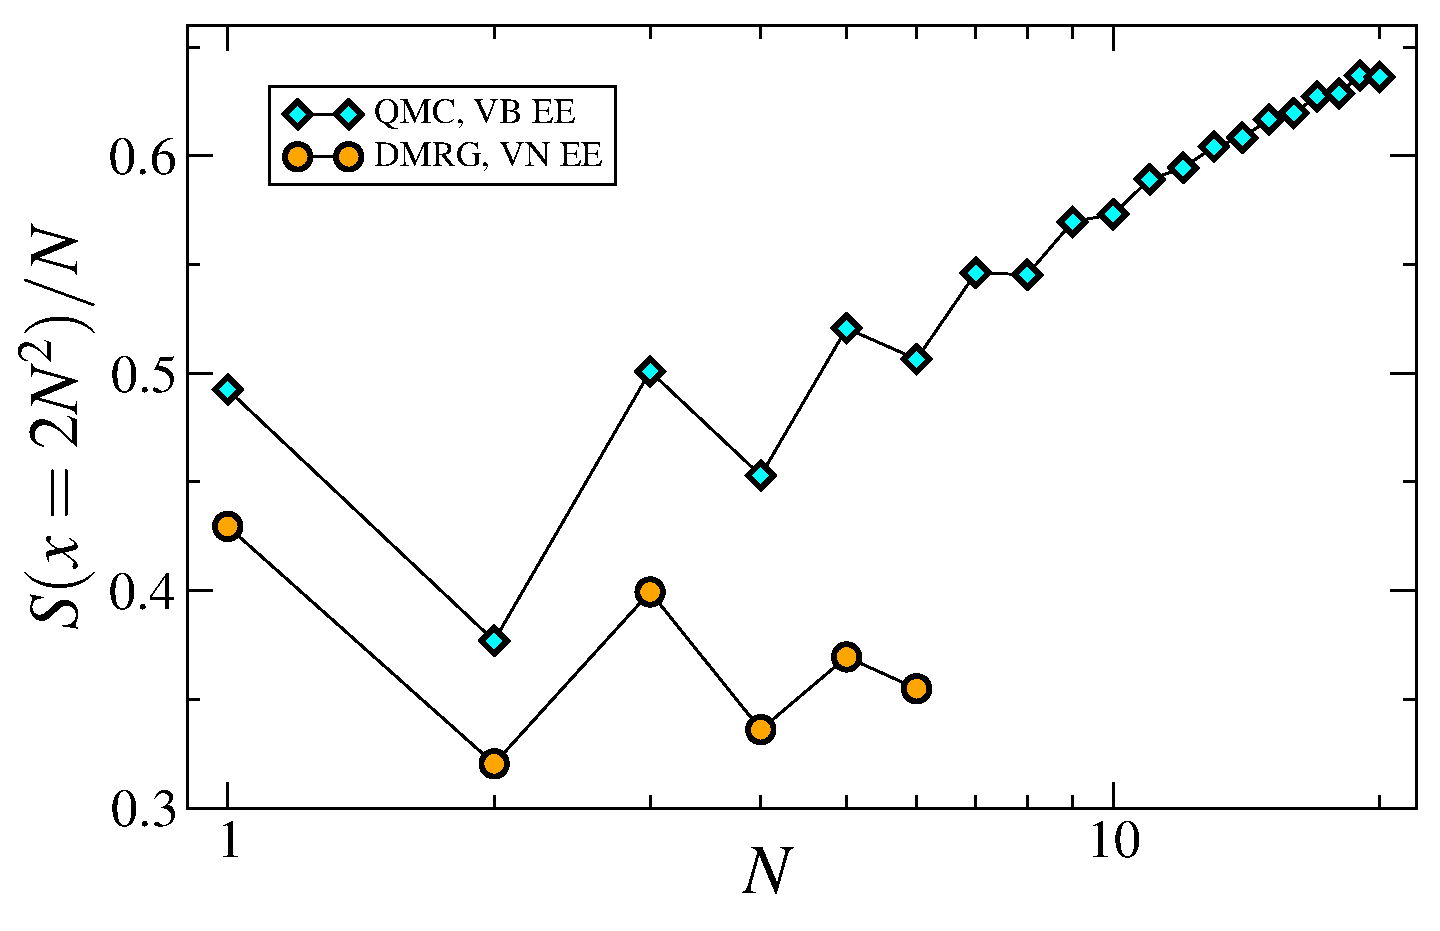
\includegraphics[width=3in]{fig4.eps} \caption{(color
online) The VB and VN entanglement entropies (taken such that the region A
includes $2N^2$ sites) normalized by N, the number of legs.  All ladders
have 100 sites per leg.  \label{zigzag}}} \end{figure}

{\it Discussion.}-- In this paper, we have compared scaling properties of
the valence bond (VB) entanglement entropy (EE) defined in
Refs.~\cite{Alet,Chh} to the von Neumann (VN) entanglement entropy in the
spin 1/2 Heisenberg model on one-dimensional and multi-leg ladder
geometries.  Both entropy measurements were evaluated using large-scale
numerical simulations; the VN EE with DMRG (which is restricted to 1D or
seven-leg and less open boundary ladders), and valence-bond basis QMC,
which can access the VB EE on any lattice dimension or geometry.  In 1D,
we find that the VB mimics the behavior of the VN EE closely, although
using the definition of Eq.~\eqref{VBEE}, is less than the VN EE for
periodic 1D Heisenberg chains, and greater than the VN EE for open chains.
In addition, fits to 1D conformal field theory, which are excellent for
the VN entropy calculated via DMRG, appear to deviate significantly for
the VB EE in the large chain-size limit, approaching some $c<1$ for both
boundary conditions examined here.

On multi-leg ladder systems with open boundaries, the VB EE is
systematically greater than the VN EE, a discrepancy which grows as the
number of legs in increased.  Defining the boundary between the two
entangled regions as being bipartitioned by a cut across all legs, we can
evaluate an ``area law'' in the ladder geometries.  The VN EE measured by
DMRG adheres to the area law in the large-leg limit, whereas the VB EE
measured by QMC reproduces a multiplicative log correction found in
Refs.~\cite{Alet,Chh} for the N\'eel groundstate of the 2D Heisenberg
model.

This work has elucidated the relationship between the VB and VN EE.
Although clearly a good measurement of entanglement readily accessible to
numerical simulations in 2D and higher, the VB EE does not provide a bound
on the VN EE, unlike other entropic measures such as Renyi entropies.
Other properties of the VN EE, such as its adherence to an area law, are
reproduced in the groundstates of some gapped systems \cite{Alet,Chh},
however in the case of the N\'eel groundstate of the 2D Heisenberg model,
unphysical multiplicative logarithmic corrections appear in the VB EE,
which are not caused by gapless excitations or algebraically decaying
correlations, but simply by the valence-bond length distribution ({\bf we
need to justify this in the text}).  The presence of this correction must
be taken into account in proposals to use the VB EE for such important
future tasks such as characterizing topological phases using entanglement
entropy, or studying universality at quantum phase transitions.

{\it Acknowledgements.}-- The authors thank I. Affeck, J. Berlinsky, A.
Del Maestro and E. Sorensen for useful discussions.  Support for this work
was provided by NSERC of Canada.


\bibliography{VB_biblio}


\end{document}
